%% ----------------------------------------------------------------
%% Designs.tex
%% ---------------------------------------------------------------- 
\chapter{Model Designs} \label{Chapter:Designs}

Tensorflow 2 with Keras API is chosen to accomplish the design of neural networks and train them.
GPU is used to accelerate the training process. Detailed development tools and versions are listed in \tref{Table:version-control}.

The process of training is to use the input data and the targets in the training set to adjust the weight vectors and make the prediction results as close as possible to the target value. 
The model will iterate through the training set a number of times. Each time is called an epoch. In theory, the performance of each traversal will be better than the last epoch. 
In each epoch, the training data is divided into batches, and each batch contains $B$ input sequences, $B$ being the batch size. 
The reason to divide it into batches is to enable GPU to do parallel training, significantly saving time consumption. 
Each batch is randomly sampled from the entire training set, which can increase the randomness of the data, and reduce the model's dependence on specific batches of data. 

The early stopping method is used throughout the training process. It is a process to monitor some indicators and stop training when a certain condition is met. 
For all the model designs, the MSE is monitored and the training will stop when the loss stops decreasing for 10 epochs. 

\section{Localised Designs}

\subsection{Pure Temporal Design}

A simple LSTM model is designed to extract temporal information. A total of 19 features for each sample are used as input. 
The static features are not included since they are constant for a single location.
\tref{Table:simplelstm-features} gives all the features used and the positions they are at. In the process of training, all the features are treated as \verb|float32|.
The types in the table are just an indication of what kind of values they might be. 

\begin{table}[!htb]
    \centering
    \begin{tabular}{c|cc|c|cc}
    \toprule
    features & position & type & features & position & type \\
    \midrule
    \verb|year| & 0 & float &  \verb|is_morning_rush_hour| & 15 & bool\\
    \verb|month| & 1-12 & bool & \verb|is_evening_rush_hour| & 16 & bool \\
    \verb|is_weekday| & 13 & bool & \verb|is_missing| & 17 & int \\
    \verb|is_workday| & 14 & bool & \verb|travel_time| & 18 & float \\
    
    \bottomrule
    \end{tabular}
    \caption{Dimensions of samples for a single link}
    \label{Table:simplelstm-features}
\end{table}

\fref{Figure:simplelstm-structure} shows the structure of the model. It is a sequential model in which each layer is connected one after another. 

\begin{figure}[!htb]
    \centering
    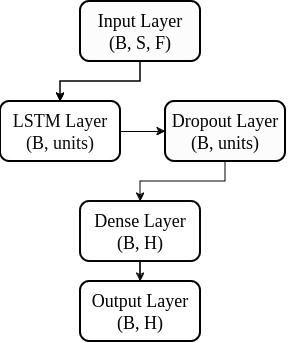
\includegraphics[width=6cm]{simplelstm-structure}
    \caption{Basic structure of the simple LSTM model, with the notes of the dimension changes}
    \label{Figure:simplelstm-structure}
\end{figure}

The input layer feeds the input sequence into the LSTM layer, with a dimension of $\mathbf{X} \in \mathbb{R}^{B\times 30\times 19}$. 
The LSTM layer with different values of units will then extract temporal information for each sequence, and change the dimension to $(B\times \mathrm{units})$.
The unit is a parameter that indicates the number of LSTM nodes in the layer. It is the length of the weight vector $\mathbf{w}$. 
Only the units in the last time frame of the sequence will be output from the LSTM layer. Those values are used to form the final targets.

To give a more powerful model, more LSTM layers could be added in series before the dropout layer. Multiple LSTM layers could increase the capacity of the model, the layer hence could capture the long-term patterns better. 
Each layer can learn feature representations at different levels of abstraction. Instead of returning the final $\mathbf{h}_t$, every output of the sequence should be returned except the last LSTM layer. 
This way, the layers could be connected sequentially.

The dropout layer randomly discards a certain amount of neurons, thereby forcing the model to have a more robust performance. 
The discard ratio can be adjusted by tuning the dropout rate. 

A dense layer is added to the end to give the correct output dimension. It is fully connected and hence has a great amount of weights to train. 
The activation function of this layer is the exponential ReLU function. 

This results in a total of 49915 trainable parameters. 
With this design, the effects on the final performance by the number of LSTM nodes, the dropout rate, and the batch size have been studied. 

\subsection{LSTM with Spatial Features}

As explained in \sref{Section:SpatialData}, features of the speed at the last time frame from the upstreams are added to the inputs. 
The resulting input dimension would now be $\mathbf{X} \in \mathbb{R}^{B\times 30\times 23}$. 
Everything else stays the same as the pure temporal model, the increase in performance by adding the spatial features would be quantified.

\section{Globalised Designs}

Another approach to predict the traffic speed is to consider the map as a whole and make predictions of every link at the same time. 
Two complicated models compared to the localised one were designed. 

The main difference between this approach from the localised designs is the sequenced data. Now the model is dealing with a total of 132 links, each link contains some statical and temporal features. 
The statical features are now in use, giving 2 additional features for every link. 
The temporal data are the features from \tref{Table:simplelstm-features}, does not change.

Combining all those together, the models now have three inputs in total: temporal inputs with a dimension of $\mathbf{X_{temp}} \in \mathbb{R}^{N\times V\times F_t}$ where $V$ stands for the number of links, $F_t$ is the feature count of the temporal data; 
statical inputs $\mathbf{X_{stat}} \in \mathbb{R}^{V\times F_s}$, where $F_s$ is the feature count of static data; and finally, the spatial inputs $\mathbf{A} \in \mathbb{R}^{V\times V}$, which is the adjacency matrix of the map. 

The model is also trained by the number of batches in each epoch, hence all three inputs need to add a dimension of batches. 
The statical and spatial inputs are broadcasted to match the dimensions.
Similar to the localised designs, the temporal inputs also need to be in sequences for LSTM layers to train. 
This makes the input shape of temporal inputs $\mathbf{X_{temp}} \in \mathbb{R}^{B\times S\times V\times F_t}$. 
This process creates a lot of duplicates of the data. Due to the memory usage restraint, a generator generates data used in each batch is used, rather than feeding the whole dataset into the model at once.  

The outputs also contain the predictions of all links. The output shape is hence $\mathbf{H} \in \mathbb{R}^{B\times H\times V}$. 
For each time frame, a prediction of the speed of every link is structured. 

\subsection{Spatio-Temporal LSTM (ST-LSTM)}

The structure of one design that can deal with spatial and temporal information is illustrated in \fref{Figure:stlstm}. 
It is a combination of the use of CNN layers and RNN layers. 

\begin{figure}[!htb]
    \centering
    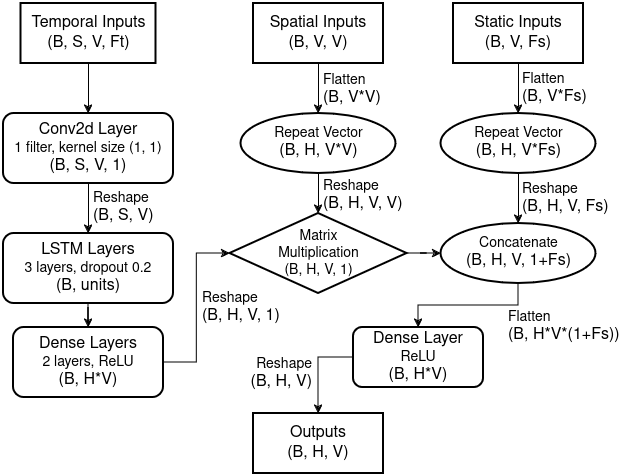
\includegraphics[width=14cm]{stlstm}
    \caption{Structure of the Spatio-Temporal LSTM design illustrated in a flowchart}
    \label{Figure:stlstm}
\end{figure}

In the sequences of the temporal data, each time frame contains two-dimensional features: $V$ and $F_t$. However, the LSTM layer can only handle one-dimensional features for one time step. 
This could be sorted by using a two-dimensional convolutional layer with 1 filter and a kernel size of (1, 1), to compress the information contained by features in $F_t$ into 1 feature. 
So now each link is related to only one feature. The LSTM layer hence can take that feature of a total of 132 links as features of the time frame. 

Now the LSTM layer is dealing with the whole map of data. It needs to be more powerful compared to ones of the localised designs. 
A three-layer LSTM sequence is used to extract temporal information. The three LSTM layers are connected sequentially, each containing 100 nodes,
The ones after using the output sequence generated from the previous layer as inputs. The final layer outputs a vector of 100 units. 

Inherit from the localised designs, two dense layers are used to match the dimension for future usage. 
The spatial inputs and static inputs are repeated first to match the target length, they are all the same across the time frames of the target. 
The processed temporal data is then multiplied with the spatial input, to merge the two data together. This is when the temporal information is combined with the spatial information.
The outcome of this stage will give a dimension of $\mathbb{R}^{B\times H\times V\times 1}$. 

The static data is then concatenated with it to extend the last dimension. Finally, a dense layer learning the statical and spatial data added is then used before the final output. 
The model contains a total of 31365780 trainable parameters, even considering 237620 parameters per link, it is still much more than the localised design. 

\subsection{GCN-LSTM}

In the ST-LSTM design, the spatial information is trained by a dense layer at the end. 
A dense layer is more effective for extracting high-level features and is suitable for data that is not affected by internal structures.
It works to extract spatial information, but it is certainly not the best choice.
Also, the input is merged into the sequenced temporal data after the extraction of temporal information by LSTM layers. 
This may cause the model to lose its vision of the spatial perspective when dealing with temporal data. 

\begin{figure}[!htb]
    \centering
    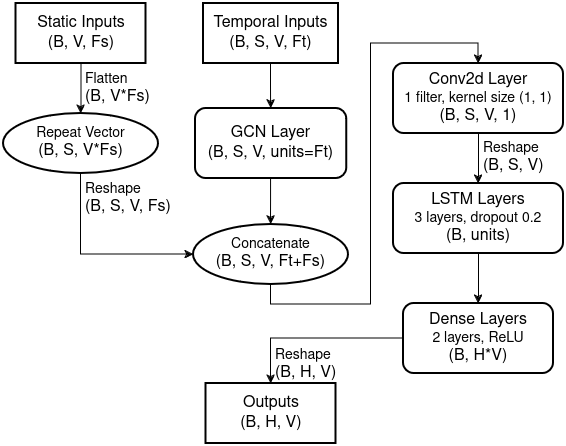
\includegraphics[width=14cm]{gcn_lstm}
    \caption{Structure of the GCN-LSTM design illustrated in a flowchart}
    \label{Figure:gcn_lstm}
\end{figure}

GCN layer is a better choice here. Since the adjacent matrix is not changing over time frames, the spatial information could be implemented into the GCN layer before training the data. 
Refering to Equation \ref{eq:gcn}, $\mathbf{D}^{-\frac{1}{2}}(\mathbf{A} + \mathbf{I})\mathbf{D}^{-\frac{1}{2}}$ is given as the model is defined.

\fref{Figure:gcn_lstm} shows the structure of the new GCN-LSTM design. 
This design is inspired by the STGCN design from \cite{Yu_2018}, which uses two temporal gated convolution layers to sandwich a spatial graph convolution layer.
In this design, the spatial inputs no longer exist since the matrix is implanted into the GCN layer. 

Before the convolutional layer and LSTM layers, the GCN layer with 19 units (which is the same amount as $F_t$) is used. 
It hence does not change the dimension of $\mathbf{X_{temp}}$, but the features are updated based on the road topology.
Along with the spatial information, the statical inputs are also merged before the extraction of the temporal information.

In this way, it should be expected to get a better performance.
In addition, there are only 2337381 trainable parameters used in total. It is significantly less than the STLSTM design, only 7.45\%.
